\documentclass[12pt] {article}
\usepackage{times}
\usepackage[margin=0.6in,bottom=1in,top=0.5in]{geometry}

\usepackage{hhline}
\usepackage{subfig}
\usepackage{graphicx}
\usepackage{amsmath}




\begin{document}

\title{Final Project - Graph Coloring - EEC289Q}
\author{Yuxin Chen and Ruolan Zeng}
\date{February 27nd, 2018}
\maketitle
%============Table========
%\begin{figure}[tbh]
% \centering    
%\begin{tabular}{ |p{4cm}|| p{2cm}|p{2cm}|p{2cm}|p{2cm}|}
% \hline
% & Processor 1 &  Processor 2  & Processor 3 & Processor 4\\ \hhline{|=|=|=|=|=|}
% \hline
% Performance          &$1.08$        &$1.425$       &\textbf{1.52}  &   \\
% \hline
%\end{tabular} 
%\caption{Metric table for the four processors}
%   \label{tab:metric}
%\end{figure} 
%============Figure========
%\begin{figure}[!tbh]
%\centering        
%   \subfloat {\includegraphics[width=0.65\textwidth]{fig2_4.png}}
%   \caption{ }
%   \label{fig:fig}
%\end{figure}

\section*{Algorithm Details:}
Generally, there are two approach to do graph coloring: 1) independent set (IDS) based 2) greedy algorithm based. In our work, we chose to use independent set (IDS) based algorithm. 
The IDS-based algorithm first assigns random number for each node in the input graph. Then the algorithm proceeds by adding the nodes with maximum random number among their neighbor (nodes they are connected to) to an independent set. Nodes in an independent set are colored with the same colors and deleted from the graph. The process continues between two phases; finding IDS and coloring the IDS and deleting it from the graph until all nodes are colored. 

\subsection*{An naive implementation}
An naive implementation: 
%\begin{figure}[!tbh]
%\centering        
%   \subfloat {\includegraphics[width=0.5\textwidth]{naive.jpg}} 
%   \caption{Overview of IDS based graph coloring.}
%   \label{fig:fig1}
%\end{figure}

Each iteration, each thread access one node, it will see first if its InIDS value (is in the independent set?) is 1, if yes, it exits, if no, it needs to see its neighbor's InIDS value and only compares the node's random number with its neighbor's whose InIDS value is 0. If it is the maximum among its neighbors, it first writes itself into independent set IDS0 (or IDS1, IDS2, dependent on the iteration), and set the node's InIDS value to 1. Then it goes to next iteration. 

So if at this iteration, a node is not included into an independent set, next iteration, it still needs to compare with its live neighbors (dead if some node are included in an independent set). This node will keep using the same neighbor list until it is added to an independent set. There is potential two improvement for this naive implementation: 
\begin{enumerate}
\item Some threads will access node that are in independent sets, then exits immediately. Since threads are executed in warps, if half of the threads in a warp exit immediately, then we wasting computing cycles and under utilize the hardware. 
\item Data reuse. Now all the memory access goes through global memory. We should think about using shared memory.
\end{enumerate}

Now just think about how to use shared memory, if we distributed nodes to different blocks, each node can load its neighbor list into shared memory and reuse it until it is added to an independent set. However, each iteration, the node also needs to know its neighbor's status (if added to IDS). If its neighbor belongs to other block, it is hard to keep data coherency among blocks. 

\section*{Communication free graph coloring}
We propose this communication free (CF) graph coloring approach:
\begin{figure}[!tbh]
\centering        
   \subfloat {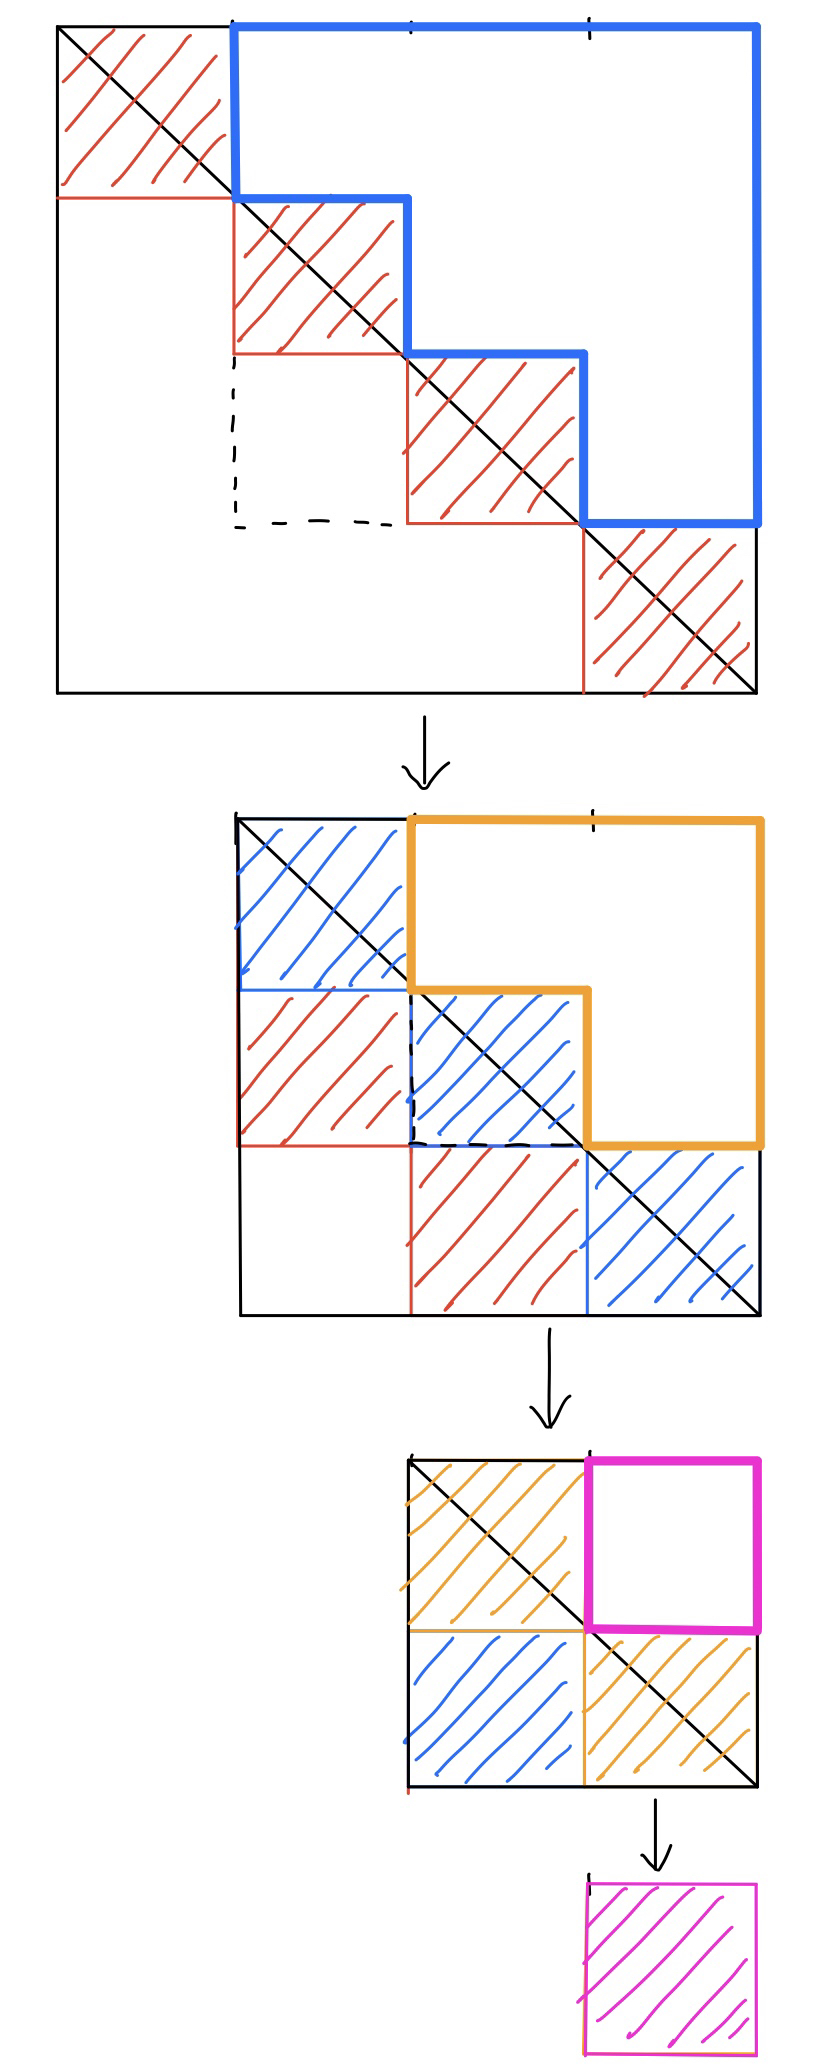
\includegraphics[width=0.25\textwidth]{comfree.jpg}}
   \caption{Overview of communication free graph coloring.}
   \label{fig:fig2}
\end{figure} 
In \ref{fig:fig2}, in the upper most matrix, the red line marked square, we call it a local block. The size of the local block will constrained by the size of shared memory and local block will run in CUDA block. Each local block will only color the nodes corresponding to their location in the matrix. We call this local graph coloring. 
When we run local graph coloring, we only color nodes based its visible neighbors, ignor the node's neighbors that are on other blocks, i.e., we don't examine the neighbor which belongs to other blocks. After each block finishes local graph coloring, the conflict can only happen between nodes that belongs to different blocks which is marked in the solid bold blue line in the uppermost matrix in \ref{fig:fig2}. Then we get the matrix covering the conflict part and run local graph coloring on this smaller matrix with its original color and set of new colors. In \ref{fig:fig2}, the second matrix is got from the uppermost matrix by finding the matrix which can best cover the conflict part (blue part). Then we run local graph coloring on the second matrix and the part marked with blue line will have no conflict. Conflicts will happen in the yellow part. We run this algorithm until there is no conflict nodes.  
Because we run local graph coloring in shared memory, it should be fast and use less color (since has less connectivity). Each block can run local graph coloring in parallel without communication. As seen from \ref{fig:fig2}, the red line marked parts in the first matrix can run in parallel, the blue line marked parts in the second matrix can run in parallel. When the conflict part is small enough to fit into a local block, we run it in a local block 

\subsection*{Potential problem with communication free graph coloring}
\begin{enumerate}
\item This algorithm might use many colors since for each phase in \ref{fig:fig2}, we use new set of color to color nodes.
\item The workload for each local block varies since each node can have different number of visible neighbors.
\item Within local block, during local graph coloring, mapping each thread a node can under utilize the hardware resource. We could like to map each thread to a neighbor to increase utilization.
\end{enumerate}
For now only the third problem we know how to solve: using scan, load balancing search and work item rank. However, for the first and second problem. We don't know yet. I even start to think this approach is not feasable at all.
Maybe for the first problem, we could try to combine greedy graph coloring to make the use of color small.

\section*{Very random Graph coloring}
In case the communication free graph coloring is unfeasible or too time-commusing which it likely to be, we plan to practice our coding and loading balacing technique on this very random graph coloring. 

Very random graph coloring is alse IDS based graph coloring. Each iteration, each node will be given a random number. each node will see, first if itself is in some IDS. If yes, it do nothing, if no, it will only check if it is the max among its neighbors. Since each iteration, a node will be assigned a new random number, eventually the node will be added to an independent set. We do this operation in a loop until all the nodes are added into independent sets.

\subsection*{Potential problem with very random graph coloring}
\begin{itemize}
\item This algorithm will also use many colors.
\item If we map each node to each thread to finish above operation, since warp is executing unit, we could under utilize the GPU. As below figure shows:
\begin{figure}[!tbh]
\centering
   \subfloat {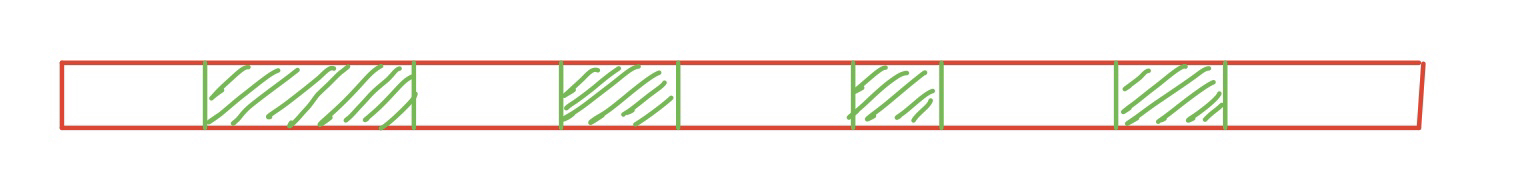
\includegraphics[width=0.35\textwidth]{nodelb.jpg}}
   \caption{Overview of communication free graph coloring.}
   \label{fig:fig3}
\end{figure}
In \ref{fig:fig3}, this array is the nodes array, and the graph part is nodes which are added to independent sets.
If the thread is assigned to the green part, it will exit.
Even we map each threads to each neighbors in CSR column\_id array, some of threads will exit imediately since the neighbors owner has been added into an independent set. 
\item If we map each node to each thread, since each node has different number of neighbors, the workload for each thread can vary.
\end{itemize}
For the second problem, we can increase the utilization by filtering out the colored nodes by doing scan.
For the third problem, there are two scheme:
\begin{itemize}
\item We could sort the nodes by its degree. For large degree nodes, we could assign a grid to process it. For medien size degree, we could assign a block to process it. For small size degree nodes, we could use warp. However this can be less desired because we launch a kernel to use grid to process large degree nodes, then another kernel to precess median degree nodes with blocks and last the kernel to process small size degree nodes. However, within each kernel, the computation is very little. Just compare and potentially set a flag. Comparing to the computation, the kernel lanuch can be significant and memory access from global memory can also be significant.
\item Instead we could map each neighbor in CSR column\_id array to a thread. Then each thread could compare the neighber with its owner and set its owner's flag if the neighbor is larger. After that, each block can synchronouse its threas and filter out the owners who are added to independent set. In previoud CUDA version, since next iteration, all nodes are assigned new random number, all blocks require synchronization. However, we can use cooperative threads in CUDA 9 to acchieve global synchronization. Then each thread remapped to the remaming neighbor and fetch its new random number and its owner's new random number, do the above iteration again until all nodes are added into an independent set.
\end{itemize}
\end{document}
